\subsection{Problema a resolver}

El siguiente ejercicio se da en el contexto de un museo donde se requiere, por cuestiones de seguridad, colocar sensores de forma tal que todo el piso del museo esté cubierto por los láser que estos emiten. Existen dos tipos de sensores: los direccionales (que emiten señales horizontales o verticales) y los bidireccionales (que emiten señales verticales y horizontales). Los valores de éstos son \$4000 y \$6000 respectivamente. Se pide también que un sensor no apunte hacia otro por que esto podría provocar que deje de funcionar, además se pide que en ciertos lugares, definidos como "importantes", haya dos láser pasando simultáneamente. El objetivo entonces es encontrar la forma de colocar los sensores de forma tal que el suelo quede completamente cubierto y que los lugares importantes queden con un laser horizontal y vertical pasando por el y además que el costo total de los sensores utilizados sea mínimo, también hay que tener en cuenta que en el museo puede haber paredes que interfieran en los láser de los sensores.

Un ejemplo de este problema es el que está provisto por la cátedra

\begin{figure}[H]
	\begin{center}
		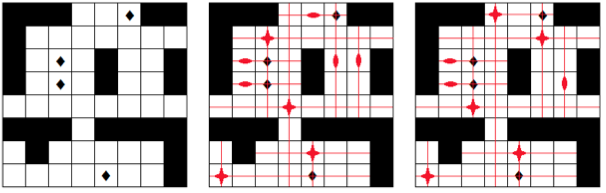
\includegraphics[width=320pt]{../imgs/ej3_ejemploCatedra.png}
	\end{center}
\caption{Un ejemplo y dos soluciones distintas.}
\end{figure}

En el ejemplo de la Figura 1 el museo se ve representado por una cuadricula donde donde los cuadrados blancos representan el suelo, los cuadrados negros representan las paredes y los cuadrados que tienen un rombo dentro representan los lugares importantes, a continuación de la imagen se muestran dos posibles soluciones al problema, en las cuales las cruces rojas representan los sensores bidireccionales, y las lineas rojas gruesas representan los sensores horizontales y verticales, desde estos se extienden lineas rojas que representan el área que cubren estos sensores con lasers.

En el primer caso el costo total es de \$44000 y la segunda solución tiene un costo de \$42000

\subsection{Resolución coloquial}

Para resolver este ejercicio usamos, como recomendación de la cátedra en el enunciado, la técnica de backtracking que consiste en probar todas las posibles combinaciones de soluciones dentro del problema hasta llegar a las válidas y guardar así la mejor de ellas usando en cada paso, criterios de parada que nos permitan deducir si las soluciones parcialmente obtenidas son candidatas a mejores soluciones o si son soluciones válidas.

El modelo de nuestro problema mapea el piso, las paredes y los lugares importantes del museo en casillas dentro de una matriz, donde cada posicion de la matriz es una "baldosa" o "casillero" en el piso, donde cada uno de estos tiene información sobre si hay algun sensor puesto o si hay algún laser pasando por encima.

El problema se resuelve recorriendo la matriz secuencialmente y en cada paso tomando una decisión sobre el casillero actual, siento esta colocar un sensor o dejar el casillero sin ningún sensor, esto genera un árbol de decisiones en el cual cada una de sus ramas representan un escenario diferente en la distribución de sensores en la matriz que representa nuestra modelo, de esta manera nos garantizamos obtener todas las posibles combinaciones de configuraciones de la matriz. Finalmente, tomamos todas estas configuraciones, chequeamos cuales son soluciones correctas y nos quedamos con la que minimiza el costo de los ContarSensores.

\subsection{Demostración de correctitud}

Sea $C$ el conjunto de configuraciones posibles de la matriz, si en cada paso puedo probar 4 opciones diferentes para cada casillero disponible, y si mi matriz mide $n*m$, entonces por combinatoria tengo $4^{n*m}$ configuraciones finales posibles de la matriz, como nuestro algoritmo hace esencialmente eso (excepto por las podas y criterios de terminación que no representan soluciones validas) podemos decir que este encuentra todas las posibles configuraciones de la matriz.

Como $C$ representa el conjunto de todas las posibles configuraciones del problema (en particular las que son solucion del problema) entonces la solución óptima, si es que existe alguna, está dentro de ese conjunto, y nuestro algoritmo debería encontrarla y devolverla.

\subsection{Complejidad del algoritmo}

Pseudocódigo:

\begin{algorithm}[H]
	\SetAlgoLined
	\caption{Algoritmo de Backtracking}
	\KwIn{Matriz $grilla$}
	\KwOut{lista sensores}
	
	Lista $casillasLibres\ \leftarrow$ ObtenerPosicionesLibres(grilla)\\

	\For{Posicion $p \in grilla$}{
		\If{p es importante}{
			RestringirPorImportantes(p)\\
		}
	}

	sensores := backtrack($grilla$, $casillasLibres$)\\

	\textbf{devolver} sensores
\end{algorithm}

\begin{algorithm}[H]
	\SetAlgoLined
	\caption{backtrack}
	\KwIn{Matriz $grilla$, Lista $casillasLibres$}
	\KwOut{}
	
	Lista $casillaActual$ := Proxima casilla libre en casillasLibres\\

	\If{Puedo poner un sensor bidireccional en $casillaActual$}{
		Restringir por láser bidireccional\\
		Saco casillaActual de casillasLibres\\
		backtrack($grilla$, $casillasLibres$)\\
	}
	\If{Puedo poner un sensor vertical en $casillaActual$}{
		Restringir por láser vertical\\
		Restringir casilleros horizontales\\
		Saco casillaActual de casillasLibres\\
		backtrack($grilla$, $casillasLibres$)\\
	}
	\If{Puedo poner un sensor horizontal en $casillaActual$}{
		Restringir por láser horizontal\\
		Restringir casilleros verticales\\
		Saco casillaActual de casillasLibres\\
		backtrack($grilla$, $casillasLibres$)\\
	}

	Dejo el casillero en blanco\\
	backtrack($grilla$, $casillasLibres$)\\

	\textbf{devolver} ContarSensores($grilla$)
\end{algorithm}

\subsection{Código fuente}

\subsection{Instancias posibles}
Para verificar la correctitud de nuestro programa, dispusimos variar estratégicamente las instancias de entrada al ejecutarlo.
\begin{itemize}
\item En primer lugar, ejecutamos el programa ingresando un único espacio libre el cual contenía un lugar importante. La idea de esto es comprobar que nuestro algoritmo devuelve -1 en el caso de que no haya solución ya que el espacio especial no podia ser cubierto por 2 láser's.\newline

\textbf{Parámetro de entrada:} 
$$3\ \ 3$$
$$0\ \ 0\ \ 0$$
$$0\ \ 2\ \ 0$$
$$0\ \ 0\ \ 0$$
\textbf{Parámetro de salida:} $$-1$$\newline
\item Por otra parte, probamos el programa cuando todo el museo es una pared y no contiene ni espacios libres ni espacios importantes, en otras palabras, el caso vacío. Lo interesante de esto es ver que nuestro algoritmo funciona en dicho caso borde y que devuelve que el problema tiene solución y que la solución es no colocar ningún láser.\newline

\textbf{Parámetro de entrada:} 
$$3\ \ 3$$
$$0\ \ 0\ \ 0$$
$$0\ \ 0\ \ 0$$
$$0\ \ 0\ \ 0$$
\textbf{Parámetro de salida:} $$0\ \ 0$$\newline
\item Un caso interesante, es ver cuando todos los espacios están libres. La idea de esto es comprobar que el algoritmo nos da la solución mas barata al problema\newline

\textbf{Parámetro de entrada:} 
$$3\ \ 3$$
$$1\ \ 1\ \ 1$$
$$1\ \ 1\ \ 1$$
$$1\ \ 1\ \ 1$$
\textbf{Parámetro de salida:} 
$$3\ \ 12000$$
$$2\ \ 0\ \ 0$$
$$2\ \ 1\ \ 2$$
$$2\ \ 2\ \ 0$$
\newline

\item Otro caso interesante, es ver cuando todos los espacios son importantes. Este es un caso particular en el cual no existe solución ya que no podrían pasar dos láser's por el mismo punto especial sin que uno de estos toque a otro láser\newline

\textbf{Parámetro de entrada:} 
$$3\ \ 3$$
$$2\ \ 2\ \ 2$$
$$2\ \ 2\ \ 2$$
$$2\ \ 2\ \ 2$$
\textbf{Parámetro de salida:} $$-1$$\newline

\item Otro caso interesante, es ir alternando entre piso y pared. Lo interesante de este caso es que no se puede aplicar ninguna poda.\newline
\textbf{Parámetro de entrada:} 
$$3\ \ 3$$
$$1\ \ 0\ \ 1$$
$$0\ \ 1\ \ 0$$
$$1\ \ 0\ \ 1$$
\textbf{Parámetro de salida:} 
$$5\ \ 20000$$
$$2\ \ 0\ \ 0$$
$$2\ \ 0\ \ 2$$
$$2\ \ 1\ \ 1$$
$$2\ \ 2\ \ 0$$
$$2\ \ 2\ \ 2$$
\newline


\item Por ultimo, esta el caso en el que tenemos los 3 tipos de casilleros, este seria el caso mas común del problema. \newline

\textbf{Parámetro de entrada:} 
$$3\ \ 3$$
$$1\ \ 1\ \ 1$$
$$1\ \ 2\ \ 0$$
$$0\ \ 0\ \ 1$$
\textbf{Parámetro de salida:} 
$$3\ \ 14000$$
$$1\ \ 0\ \ 1$$
$$2\ \ 1\ \ 0$$
$$2\ \ 2\ \ 2$$
\newline
\end{itemize}

\subsection{Testing}


